\documentclass[a4paper]{article}
\usepackage{graphicx}
\usepackage[absolute,overlay]{textpos}
\usepackage{background}
\usepackage{times}
\usepackage{lmodern}
\usepackage{geometry}
\geometry{a4paper,left=1.5cm,right=1cm,top=1cm,bottom=1cm,columnsep=0.8cm}
\usepackage{fontawesome5}
\usepackage[hidelinks]{hyperref}
\usepackage{fontspec}
\setmainfont{Arial}
\usepackage{eso-pic}
\definecolor{texcolor}{HTML}{e2e8f0}

%Ne touchez pas cette image c'est mon background tu laisse le nom comme ça.
\AddToShipoutPictureBG{ 
  
\includegraphics[width=\paperwidth,height=\paperheight]{background.jpg}
}

\newcommand{\cvsection}[1]{
\begin{tabular}{@{}p{0.26\linewidth}}
\\
\textbf{\Large #1}  \\[10pt]
\end{tabular}
}

\newcommand{\cicon}{\tikz[baseline]{\draw[fill=white] (0,0.1) circle [radius=0.25cm];}~ }

\setlength{\parindent}{0pt}

\begin{document}

%% Change le nom photo.jpg par le nom de la photo que tu as reçu.
\begin{textblock*}{4cm}(0.2cm,0.3cm) % largeur x (x, y) depuis le coin haut gauche
  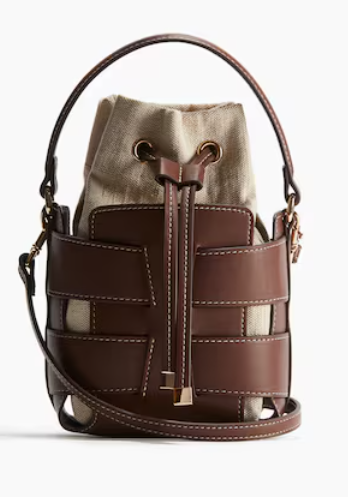
\includegraphics[width=2.5cm,clip,keepaspectratio]{94881af856a7478cadefe3e7d1cf3cce.png}
\end{textblock*}

\color{texcolor}

\begin{center}
{\fontsize{44pt}{24pt}\selectfont \textbf{Dora SARKIS}}

~

{\Large Gérante / Directrice}

~

~

\faMapMarker ~ 53 résidence Les Citronnelles  ~ ~ \faEnvelope  ~ \href{mailto:leroyalriviera@gmail.com}{leroyalriviera@gmail.com}

~


\begin{tikzpicture}
  \node[draw, fill=white, rounded corners=9pt, inner xsep=8pt, inner ysep=4pt, align=center] 
    {\color{black}\faGlobe~\href{}{ }};
\end{tikzpicture}
~ ~ 

\begin{tikzpicture}
  \node[draw, fill=white, rounded corners=9pt, inner xsep=8pt, inner ysep=4pt, align=center] 
    {\color{black}\faFigma~\href{}{ }};
\end{tikzpicture}
~ ~ 

\begin{tikzpicture}
  \node[draw, fill=white, rounded corners=9pt, inner xsep=8pt, inner ysep=4pt, align=center] 
    {\color{black}\faGithub~\href{}{ }};
\end{tikzpicture}
\end{center}

\vspace{-0.3cm}

\hspace{-1.5cm}\rule{\paperwidth}{0.4pt}

%-------------------------------------------------------------------
%                          PROFIL
%-------------------------------------------------------------------
\begin{tabular}{@{}p{0.26\linewidth}p{0.7\linewidth}}
\\
\textbf{\Large Profil} & 
Professionnelle du commerce et de l’événementiel, forte de plus de 15 ans d’expérience dans la création et la gestion d’entreprises. Fondatrice et dirigeante de plusieurs structures, elle maîtrise la gestion opérationnelle, la négociation commerciale et la relation client. Son parcours atteste d’une grande autonomie, d’un sens aigu de l’organisation et d’une rigueur administrative éprouvée. Animée par un intérêt marqué pour les questions juridiques liées aux affaires et à l’immobilier, elle recherche de nouveaux défis où son leadership pourra créer de la valeur.\\
\end{tabular}

~

\rule{\linewidth}{0.05pt}

%-------------------------------------------------------------------
%                         EDUCATION
%-------------------------------------------------------------------
\begin{tabular}{@{}p{0.26\linewidth}p{0.7\linewidth}}
\\
\textbf{\Large Education} & 
Formation en décoration événementielle \hfill {\small 2008} \\
& Centre ABC — Approfondissement des techniques de design et de mise en scène d’événements. \\[6pt]

BTS Commerce international (inachevé) \hfill {\small 2008} \\
& CNED — Bases du commerce global, de la négociation et de la logistique internationale. \\[6pt]

Baccalauréat professionnel Commerce \hfill {\small 2006} \\
& CNED — Fondamentaux de la vente, de la gestion et de la relation client. \\
\end{tabular}

~

\rule{\linewidth}{0.05pt}

%-------------------------------------------------------------------
%                        EXPERIENCE
%-------------------------------------------------------------------
\begin{tabular}{@{}p{0.26\linewidth}p{0.7\linewidth}}
\\
\textbf{\Large Experience} & 
\textbf{Gérante} \hfill {\small 2019--Présent} \\[6pt]
& \textbf{Boutique à Pointe-à-Pitre \& gestion de locaux commerciaux} \\[6pt]
& Dirige la boutique au quotidien et supervise la gestion de plusieurs locaux commerciaux. \\[6pt]
& Gère la relation client et les négociations avec rigueur et sens de l’organisation. \\[12pt]

& \textbf{Directrice} \hfill {\small 2012--2018} \\[6pt]
& \textbf{Salle de spectacle} \\[6pt]
& Piloté le management des équipes, l’organisation d’événements et la gestion administrative. \\[6pt]
& Développé une offre événementielle répondant aux attentes du public et des partenaires. \\[12pt]

& \textbf{Gérante fondatrice} \hfill {\small 2008} \\[6pt]
& \textbf{Joykiss} \\[6pt]
& Créé et développé une boutique spécialisée mariage avec services de wedding planning et design. \\[6pt]
& Assuré la gestion, la négociation fournisseur et le développement de l’offre produits. \\
\end{tabular}

~

\rule{\linewidth}{0.05pt}

%-------------------------------------------------------------------
%                          SKILLS
%-------------------------------------------------------------------
\begin{tabular}{@{}p{0.26\linewidth}p{0.18\linewidth}p{0.18\linewidth}p{0.18\linewidth}}
\\
\textbf{\Large Skills} & 
\cicon Gestion d’entreprise & \cicon Négociation commerciale & \cicon Relation client \\[6pt]
& 
\cicon Organisation d’événements & \cicon Management administratif & \cicon Autonomie \\[6pt]
& 
\cicon Rigueur & \cicon Sens de l’organisation & \cicon Droit commercial \\[6pt]
& 
\cicon Droit des affaires & \cicon Droit immobilier & \cicon  \\
\end{tabular}

\end{document}